%==============================================================================
%  MATH 231 -- Linear Algebra I (Queens College, Fall 2026)
%  VECTOR CALCULUS UNIT, PART 1 -- Derivatives, and the Gradient in the Plane
%
%  A NEW UNIT.  Section numbering restarts at 1 here.  It does NOT continue from
%  the vector unit (Sec. 1-24), the computational unit (Sec. 1-23), or the
%  matrix unit (Sec. 1-9).  Every cross-reference OUT of this unit must name the
%  unit, since a bare "Sec. 5" is now ambiguous four ways.  The front matter
%  states that for students.
%
%  THIS UNIT IS SPLIT ACROSS TWO DOCUMENTS, numbered continuously:
%      Part 1  MATH231_veccalc_1_derivatives_and_the_gradient   Sections 1-9
%      Part 2  MATH231_veccalc_2_n_dimensions_and_the_hessian   Sections 10-15
%  Part 2 opens with \setcounter{section}{9}.
%
%  WHERE THE SPLIT FALLS, AND WHY.  Part 1 is deliberately confined to
%  f : R^2 -> R and assumes ONLY the lectures actually delivered so far --
%  vectors Parts 1, 2 and 3, plus complex numbers.  In particular:
%
%    - NO STANDARD BASIS.  e_j lives in vector unit Sec. 16 (vectors Part 4),
%      which has not been lectured.  So the partial derivative is defined here
%      coordinate-wise -- f(x+h, y) and f(x, y+h) -- and NOT as a step h*e_j.
%      Part 2 introduces e_j and re-states the definition with it, which is the
%      form that generalises.  If this file is edited, keep e_j out of it.
%    - NO R^n.  Every signature in Part 1 is R^2 -> R.  The lift to n
%      dimensions is the opening move of Part 2.
%
%  STATUS: complete.  Sections 1-9.
%
%  WHY THE CALCULUS REVIEW IS HERE AT ALL.  Everything through Sec. 4 is
%  MATH 141 material.  It is restated rather than assumed because Sec. 6 defines
%  the partial derivative as a one-variable derivative taken along a coordinate
%  direction -- so the one-variable definition has to be fresh and in the same
%  notation, not merely "seen last year".  Sec. 1.1 and Sec. 6.1 are deliberately
%  the same limit with one substitution between them.
%
%  SEC. 2 HOLDS ONLY the structural rules and the six trigonometric ones.  The
%  exponential/logarithm derivatives are deliberately absent: they are DERIVED
%  in Sec. 4, and Sec. 2 says so explicitly rather than quoting the answers
%  first and justifying them later.  Sec. 3 supplies the algebraic properties
%  (E1-E5, L1-L5) that Sec. 4.1 and Sec. 4.3 actually consume.
%
%  SEC. 8 IS THE CENTREPIECE and is now PROVED, not asserted.  The chain is:
%    8.1  directional derivative introduced as an idea, then as the limit
%         (eq:dirderiv) with step h*u; both partials fall out as special cases.
%    8.2  D_u f = <grad f, u>, motivated by adding the two coordinate effects.
%         This is flagged as a motivation, NOT a proof -- Sec. 9.2's closing
%         remark discharges it from the linear approximation.  Keep that
%         ordering honest if this is edited.
%    8.3  the maximisation: <grad f, u> = ||grad f|| ||u|| cos(theta)
%         = ||grad f|| cos(theta); only cos(theta) varies; maximal at theta = 0;
%         u = grad f / ||grad f|| realises it and returns ||grad f||.  Hence
%         ascent direction, hence steepest ascent.  The rmk collects theta = pi
%         (steepest descent) and theta = pi/2 (the level curves) from the SAME
%         equation, at no extra cost.
%    8.4  gradient descent, with the iterate x_{k+1} = x_k - alpha grad f(x_k).
%
%  SEC. 6.2 (the slice picture) is the geometric support for the partial
%  derivative: cut the surface with the plane y = b, get a one-variable curve,
%  and df/dx is the slope of ITS tangent.  It is also what Sec. 9.2's
%  tangent-plane remark points back to.
%
%  LANGUAGE DELIBERATELY AVOIDED: "continuously differentiable", "smooth",
%  "class C^1".  The worked functions all satisfy every hypothesis anyone could
%  want; saying so would cost a definition the course has not paid for.  Keep
%  the examples clean rather than hedged.
%
%  VECTOR-UNIT CITATIONS USED HERE, all from lectures already delivered:
%      Sec. 2      the Euclidean norm
%      Sec. 6      function notation f : A -> B
%      Sec. 11.3   the dot product, and <u,v> = ||u|| ||v|| cos(theta)
%      Sec. 11.6   <u,u> = ||u||^2
%      Sec. 11.7   the orthogonality test
%      Sec. 12.1   normalisation and unit vectors
%  (Two citations in the pre-split draft were wrong and are corrected here: the
%  norm is Sec. 2, not Sec. 11.9, and the cosine formula is Sec. 11.3, not
%  Sec. 11.6.)
%
%  AUDIENCE: distributed to students.  No instructor-facing apparatus.
%
%  Compile with pdflatex (standard TeX Live packages only; uses tikz).
%==============================================================================
\documentclass[11pt]{article}

\usepackage[margin=1in]{geometry}
\usepackage{amsmath,amssymb,amsthm}
\usepackage[dvipsnames]{xcolor}
\usepackage{enumitem}
\usepackage{booktabs}
\usepackage{array}
\usepackage[hidelinks]{hyperref}
\usepackage{titlesec}
\usepackage{needspace}
\usepackage{tikz}
\usetikzlibrary{arrows.meta,calc}

%------------------------------------------------------------------ style ----
\titleformat{\section}{\large\bfseries\sffamily}{\thesection.}{0.6em}{}
\titleformat{\subsection}{\normalsize\bfseries\sffamily}{\thesubsection.}{0.5em}{}
\titlespacing*{\section}{0pt}{14pt}{6pt}

\theoremstyle{plain}
\newtheorem{thm}{Theorem}[section]

\theoremstyle{definition}
\newtheorem{defn}{Definition}[section]
\newtheorem{ex}{Example}[section]
\theoremstyle{remark}
\newtheorem*{rmk}{Remark}
\newtheorem*{warn}{A common confusion}

\newcommand{\lookahead}{\par\smallskip\noindent
  \textbf{\sffamily\textcolor{RoyalBlue}{Looking ahead.}}\ \ignorespaces}
\newcommand{\lookback}{\par\smallskip\noindent
  \textbf{\sffamily\textcolor{ForestGreen}{From the vector unit.}}\ \ignorespaces}

%--------------------------------------------------------------- notation ----
\newcommand{\R}{\mathbb{R}}
\newcommand{\vc}[1]{\mathbf{#1}}
\newcommand{\norm}[1]{\lVert #1\rVert}
\newcommand{\ip}[2]{\langle #1,\, #2\rangle}
\newcommand{\grad}{\nabla}
\newcommand{\pd}[2]{\frac{\partial #1}{\partial #2}}
\newcommand{\dd}[2]{\frac{d #1}{d #2}}
\newcommand{\mt}[1]{\mathbf{#1}}          % matrices: bold upper case
\newcommand{\T}{^{\mathsf{T}}}            % transpose
\newcommand{\pdd}[3]{\frac{\partial^{2} #1}{\partial #2\,\partial #3}}

%------------------------------------------------------------- tikz helpers --
\tikzset{
  axisline/.style = {->, gray!75, thin},
  curveln/.style  = {RoyalBlue, very thick},
  vecarr/.style   = {-{Stealth[length=2.6mm,width=2.0mm]}, very thick}
}

\title{\vspace{-1.2cm}\textbf{\sffamily MATH 231 -- Linear Algebra I}\\[4pt]
       {\large\sffamily The Vector Calculus Unit, Part 1 \textbullet\
        Derivatives, and the Gradient in the Plane}\\[2pt]
       {\normalsize\sffamily Kiely Hall 326 \textbullet\
        Instructor: Kevin Bedoya}}
\author{}
\date{}

\begin{document}
\maketitle
\vspace{-1.6cm}

\noindent\textbf{About this document.} This opens a unit on calculus in several
variables. It begins with a review of one-variable differentiation --- material
from MATH~141 --- not as a courtesy, but because the central definition of
\S6 turns out to be the one-variable definition with a single substitution made
inside it. Having that definition fresh, and in the same notation, is what makes
the new one read as a small change rather than a new idea.

Everything after \S4 concerns functions of \emph{two} variables,
$f:\R^{2}\to\R$. That is not the general case, and it is not meant to be. Two
variables is where every idea in the subject can be drawn on a page, and the
plane is the space the vector unit has been building all semester. Part 2 of
this unit lifts the whole of \S5--\S9 to $\R^{n}$, where the pictures stop and
the formulas do not change.

\begin{warn}[Section numbers restart]
This unit numbers its sections from $1$ again. They do \emph{not} continue from
the vector unit ($\S1$--$\S24$), the computational unit, or the matrix unit, all
of which also start at $1$. A bare ``\S5'' below means \S5 \emph{of this unit};
whenever we point at another we will name it. Part 2 of this unit continues the
numbering from \S10, so a reference to \S12 there is not a reference to the
vector unit's \S12.
\end{warn}

\medskip
\noindent\textbf{Assumed.} From MATH~141: limits, and differentiation of
one-variable functions. From the vector unit --- all of it from lectures already
given --- $\R^{2}$ and its vectors (\S1, \S5); the Euclidean norm (\S2);
function notation $f:A\to B$ (\S6); the dot product and the identity
$\ip{\vc{u}}{\vc{v}}=\norm{\vc{u}}\norm{\vc{v}}\cos\theta$ (\S11.3); the
orthogonality test (\S11.7); and normalisation into a unit vector (\S12.1).
Nothing from vectors Part 4 or Part 5 is used, and neither is the matrix unit.

\medskip
\noindent\textbf{What you should be able to do afterwards.} State the definition
of the derivative and use the standard rules; state the algebraic properties of
$e^{x}$ and $\ln x$ and explain why the two lists mirror each other; derive
$\tfrac{d}{dx}\ln x$ from the definition and $\tfrac{d}{dx}e^{x}$ two ways; read
the signature $f:\R^{2}\to\R$ and give examples; define the two partial
derivatives as limits, compute them, and say what they are on the surface
$z=f(x,y)$; say what kind of object a partial derivative is; assemble the
partials into the gradient; define the directional derivative and compute it as
$\ip{\grad f}{\vc{u}}$; show that the rate of change is greatest along the
gradient and explain why that makes $\grad f$ the direction of steepest ascent;
say what $-\grad f$ is and how gradient descent uses it; and write the linear
approximation of a function of one variable and of two.
%==============================================================================
\section{The derivative, in one variable}
%==============================================================================

%------------------------------------------------------------------------------
\subsection{The definition}
%------------------------------------------------------------------------------
\begin{defn}[Derivative]
Let $f:\R\to\R$. The \textbf{derivative} of $f$ at $x$ is
\begin{equation}\label{eq:deriv}
  f'(x) \;=\; \lim_{h\to0}\frac{f(x+h)-f(x)}{h},
\end{equation}
provided the limit exists. When it does, $f$ is called \textbf{differentiable}
at $x$.
\end{defn}

\noindent The quotient inside the limit is the slope of the line through the two
points $(x,f(x))$ and $(x+h,f(x+h))$ --- a \emph{secant} line. As $h$ shrinks,
the second point slides toward the first and the secant pivots. The derivative
is the slope it settles on: the slope of the tangent line at $x$, and the
instantaneous rate at which $f$ changes there.

\begin{center}
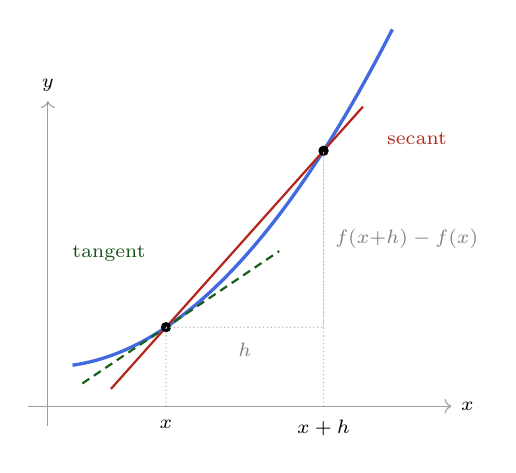
\begin{tikzpicture}[scale=1.25]
  \draw[axisline] (-0.2,0) -- (4.1,0) node[right,font=\scriptsize,black]{$x$};
  \draw[axisline] (0,-0.2) -- (0,3.1) node[above,font=\scriptsize,black]{$y$};
  \draw[curveln,domain=0.25:3.5,smooth,samples=80]
        plot (\x,{0.28*\x*\x + 0.4});
  % points
  \coordinate (P) at (1.2,0.8032);
  \coordinate (Q) at (2.8,2.5952);
  % secant, extended
  \draw[BrickRed,thick] ($(P)!-0.35!(Q)$) -- ($(P)!1.25!(Q)$);
  % tangent at P, slope 0.672
  \draw[ForestGreen!70!black,thick,densely dashed]
        (0.35,{0.8032-0.672*0.85}) -- (2.35,{0.8032+0.672*1.15});
  \fill[black] (P) circle (1.5pt);
  \fill[black] (Q) circle (1.5pt);
  % guides
  \draw[gray!55,densely dotted] (1.2,0) -- (P);
  \draw[gray!55,densely dotted] (2.8,0) -- (Q);
  \draw[gray!55,densely dotted] (P) -- (2.8,0.8032);
  \draw[gray!55,densely dotted] (2.8,0.8032) -- (Q);
  \node[below,font=\scriptsize] at (1.2,-0.04) {$x$};
  \node[below,font=\scriptsize] at (2.8,-0.04) {$x+h$};
  \node[below,font=\scriptsize,gray] at (2.0,0.74) {$h$};
  \node[right,font=\scriptsize,gray] at (2.82,1.70) {$f(x{+}h)-f(x)$};
  \node[font=\scriptsize,BrickRed] at (3.75,2.72) {secant};
  \node[font=\scriptsize,ForestGreen!60!black] at (0.62,1.55) {tangent};
\end{tikzpicture}
\end{center}

%------------------------------------------------------------------------------
\subsection{Notation}
%------------------------------------------------------------------------------
The same object is written several ways, and all of them appear in practice:
\[
  f'(x),
  \qquad
  \dd{f}{x},
  \qquad
  \dd{y}{x},
  \qquad
  \frac{d}{dx}f(x) .
\]
The last form is useful because $\tfrac{d}{dx}$ reads as an \emph{instruction}
--- ``differentiate what follows with respect to $x$'' --- which is how it is
used in \S4.2.

%==============================================================================
\section{The rules}
%==============================================================================
Computing every derivative from \eqref{eq:deriv} would be unbearable, so the
limit is evaluated once for each basic function and once for each way of
combining functions. What follows is the resulting catalogue. Throughout, $c$ is
a constant and $f,g$ are differentiable.

%------------------------------------------------------------------------------
\subsection{Structural rules}
%------------------------------------------------------------------------------
These say how differentiation interacts with the ways functions are built out of
other functions.

\begin{center}
\renewcommand{\arraystretch}{1.75}
\begin{tabular}{@{}l l l@{}}
\toprule
\textbf{Rule} & \textbf{Statement} & \textbf{Notes} \\
\midrule
Constant & $\dfrac{d}{dx}\,c = 0$
  & a flat graph has slope $0$ \\
Constant multiple & $\dfrac{d}{dx}\,\bigl[c\,f(x)\bigr] = c\,f'(x)$
  & scalars pass through \\
Sum / difference & $\dfrac{d}{dx}\,\bigl[f(x)\pm g(x)\bigr]=f'(x)\pm g'(x)$
  & term by term \\
Power & $\dfrac{d}{dx}\,x^{n} = n\,x^{\,n-1}$
  & any real $n$ \\
Product & $\dfrac{d}{dx}\,\bigl[f(x)g(x)\bigr]=f'(x)g(x)+f(x)g'(x)$
  & \emph{not} $f'g'$ \\
Quotient & $\dfrac{d}{dx}\dfrac{f(x)}{g(x)}
            =\dfrac{f'(x)g(x)-f(x)g'(x)}{\bigl[g(x)\bigr]^{2}}$
  & order of the numerator matters \\
Chain & $\dfrac{d}{dx}\,f\bigl(g(x)\bigr)=f'\bigl(g(x)\bigr)\,g'(x)$
  & outer at inner, times inner \\
\bottomrule
\end{tabular}
\end{center}

\noindent The first three together say that differentiation is
\emph{linear}: it distributes across sums and lets constants through. That word
is worth registering --- it is the same property, in the same sense, that the
vector unit attached to other operations, and it will return when the gradient
appears.

%------------------------------------------------------------------------------
\subsection{Trigonometric functions}
%------------------------------------------------------------------------------
\begin{center}
\renewcommand{\arraystretch}{1.6}
\begin{tabular}{@{}l l @{\qquad\qquad} l l@{}}
\toprule
\textbf{Function} & \textbf{Derivative} &
\textbf{Function} & \textbf{Derivative} \\
\midrule
$\sin x$ & $\cos x$              & $\csc x$ & $-\csc x\cot x$ \\
$\cos x$ & $-\sin x$             & $\sec x$ & $\sec x\tan x$ \\
$\tan x$ & $\sec^{2}x$           & $\cot x$ & $-\csc^{2}x$ \\
\bottomrule
\end{tabular}
\end{center}

\noindent A pattern worth using as a memory aid: every co-function ---
$\cos$, $\csc$, $\cot$ --- picks up a minus sign.

\noindent The exponential and the logarithm are missing from these tables on
purpose. Their derivatives are not quoted here; they are derived in \S4.

%==============================================================================
\section{The exponential and the logarithm}
%==============================================================================
Before differentiating these two, their algebra is worth setting out --- partly
because \S4.1 uses it, and partly because the two lists are the same list read
in a mirror.

%------------------------------------------------------------------------------
\subsection{The exponential function}
%------------------------------------------------------------------------------
The function $\exp(x)=e^{x}$ has domain $\R$ and range $(0,\infty)$: it is
\emph{never} zero or negative, no matter what is fed to it. It is strictly
increasing.

\begin{center}
\renewcommand{\arraystretch}{1.55}
\begin{tabular}{@{}l l l@{}}
\toprule
 & \textbf{Property} & \textbf{In words} \\
\midrule
\textbf{E1} & $e^{0}=1$                       & the exponential of nothing is one \\
\textbf{E2} & $e^{a+b}=e^{a}\,e^{b}$          & sums become products \\
\textbf{E3} & $e^{a-b}=\dfrac{e^{a}}{e^{b}}$  & differences become quotients \\
\textbf{E4} & $\bigl(e^{a}\bigr)^{b}=e^{ab}$  & powers multiply the exponents \\
\textbf{E5} & $e^{-a}=\dfrac{1}{e^{a}}$       & negation inverts \\
\bottomrule
\end{tabular}
\end{center}

\noindent E2 is the essential one; E3 and E5 are consequences of it.

%------------------------------------------------------------------------------
\subsection{The natural logarithm}
%------------------------------------------------------------------------------
The function $\ln x$ has domain $(0,\infty)$ and range $\R$ --- exactly the
exponential's domain and range, exchanged. That is the first sign that the two
are inverses.

\begin{center}
\renewcommand{\arraystretch}{1.55}
\begin{tabular}{@{}l l l@{}}
\toprule
 & \textbf{Property} & \textbf{In words} \\
\midrule
\textbf{L1} & $\ln 1 = 0$                            & mirrors E1 \\
\textbf{L2} & $\ln(ab)=\ln a+\ln b$                  & products become sums \\
\textbf{L3} & $\ln\dfrac{a}{b}=\ln a-\ln b$          & quotients become differences \\
\textbf{L4} & $\ln\bigl(a^{r}\bigr)=r\ln a$          & exponents come down in front \\
\textbf{L5} & $\ln e = 1$                            & the base is its own unit \\
\bottomrule
\end{tabular}
\end{center}

%------------------------------------------------------------------------------
\subsection{They are inverses}
%------------------------------------------------------------------------------
The two functions undo each other:
\begin{equation}\label{eq:inverse}
  \ln\bigl(e^{x}\bigr)=x \quad\text{for all } x\in\R,
  \qquad
  e^{\ln x}=x \quad\text{for all } x>0 .
\end{equation}

\noindent This is what explains the parallel between the two tables. Read E1
through E4 backwards and they become L1 through L4: E2 says $e$ turns addition
into multiplication, so its inverse must turn multiplication back into addition,
which is L2. The logarithm laws are not a second set of facts to memorise --- they
are the exponential laws seen from the other side.

\begin{warn}[$\ln$ of a sum]
L2 converts the log of a \emph{product} into a sum. There is no corresponding
rule for the log of a sum: $\ln(a+b)$ does not simplify, and in particular it is
not $\ln a+\ln b$. Check it once with $a=b=1$: $\ln 2\approx0.693$, while
$\ln1+\ln1=0$.
\end{warn}

%==============================================================================
\section{Deriving the two derivatives}
%==============================================================================
These two derivatives were deliberately left out of the tables in \S2. Here they
are earned instead. The order matters: the logarithm is done first, from the
definition alone, and the exponential then follows from it.

%------------------------------------------------------------------------------
\subsection{The natural logarithm, from the definition}
%------------------------------------------------------------------------------
Let $f(x)=\ln x$ with $x>0$. Apply \eqref{eq:deriv} directly:
\[
  f'(x)
  \;=\;\lim_{h\to0}\frac{f(x+h)-f(x)}{h}
  \;=\;\lim_{h\to0}\frac{\ln(x+h)-\ln x}{h} .
\]
The numerator is a difference of logarithms, so L3 folds it into one:
\[
  \;=\;\lim_{h\to0}\frac{1}{h}\,\ln\!\left(\frac{x+h}{x}\right)
  \;=\;\lim_{h\to0}\frac{1}{h}\,\ln\!\left(1+\frac{h}{x}\right) .
\]
Now use L4 in reverse --- a coefficient in front of a logarithm can be pushed up
into the exponent --- moving the $1/h$ inside:
\[
  \;=\;\lim_{h\to0}\ln\!\left[\left(1+\frac{h}{x}\right)^{1/h}\right]
  \;=\;\ln\!\left[\lim_{h\to0}\left(1+\frac{h}{x}\right)^{1/h}\right] .
\]
Moving the limit inside $\ln$ is legitimate because $\ln$ is continuous, and a
continuous function may be evaluated at the limit of its input.

The remaining limit is a standard one. Substituting $u=h/x$, so that $u\to0$ as
$h\to0$ and $1/h=1/(ux)$,
\[
  \lim_{h\to0}\left(1+\frac{h}{x}\right)^{1/h}
  =\lim_{u\to0}\Bigl[(1+u)^{1/u}\Bigr]^{1/x}
  = e^{1/x},
\]
using $\lim_{u\to0}(1+u)^{1/u}=e$, which is one of the standard definitions of
$e$. Therefore
\[
  f'(x)=\ln\bigl(e^{1/x}\bigr)=\frac{1}{x},
\]
the last step by \eqref{eq:inverse}. \qquad$\blacksquare$

%------------------------------------------------------------------------------
\subsection{The exponential, by implicit differentiation}
%------------------------------------------------------------------------------
With $\tfrac{d}{dx}\ln x=1/x$ in hand, the exponential costs three lines. Let
\[
  y=e^{x} .
\]
Take the logarithm of both sides, which by \eqref{eq:inverse} gives
\[
  \ln y = x .
\]
Differentiate both sides with respect to $x$. The right side gives $1$. The left
side is a function of $y$, which is itself a function of $x$, so the chain rule
applies:
\[
  \frac{d}{dx}\bigl[\ln y\bigr] = \frac{d}{dx}\bigl[x\bigr]
  \qquad\Longrightarrow\qquad
  \frac{1}{y}\,\dd{y}{x} = 1 .
\]
Solving for the derivative and substituting back,
\[
  \dd{y}{x} = y = e^{x} . \qquad\blacksquare
\]

\noindent This technique --- differentiating an equation in which $y$ is not
isolated, then solving for $dy/dx$ --- is \textbf{implicit differentiation}. It
works here because writing $\ln y=x$ converts a hard derivative into an easy
one at the cost of an extra chain-rule factor.

%------------------------------------------------------------------------------
\subsection{The exponential, from the definition}
%------------------------------------------------------------------------------
The same result comes out of \eqref{eq:deriv}. Let $f(x)=e^{x}$:
\[
  f'(x)=\lim_{h\to0}\frac{e^{x+h}-e^{x}}{h} .
\]
By E2, $e^{x+h}=e^{x}e^{h}$, so $e^{x}$ is a common factor of the numerator:
\[
  =\lim_{h\to0}\frac{e^{x}e^{h}-e^{x}}{h}
  =\lim_{h\to0}\frac{e^{x}\bigl(e^{h}-1\bigr)}{h}
  = e^{x}\lim_{h\to0}\frac{e^{h}-1}{h} .
\]
The factor $e^{x}$ does not involve $h$, so it passes outside the limit. What
remains is the standard identity
\begin{equation}\label{eq:explimit}
  \lim_{h\to0}\frac{e^{h}-1}{h} = 1,
\end{equation}
which gives $f'(x)=e^{x}$. \qquad$\blacksquare$

\begin{rmk}
It is worth being clear about what this second derivation does and does not
establish. Setting $x=0$ in \eqref{eq:deriv} for $f(x)=e^{x}$ turns it into
exactly \eqref{eq:explimit} --- so the identity \emph{is} the statement that
$f'(0)=1$. The argument therefore does not conjure the derivative from nothing;
it shows that the derivative everywhere follows from its value at the single
point $x=0$. That is a real statement, and a strong one: the exponential is
pinned down completely by its slope at the origin. The derivation in \S4.2 is
the one that stands independently, resting on \S4.1.
\end{rmk}

%==============================================================================
\section{Functions of two variables}
%==============================================================================

%------------------------------------------------------------------------------
\subsection{The signature}
%------------------------------------------------------------------------------
Everything so far has concerned $f:\R\to\R$ --- one number in, one number out.
Almost nothing worth computing has that shape.

\lookback The notation $f:A\to B$ was fixed in \S6 of the vector unit: the set
before the arrow is what the function consumes, the set after it is what the
function produces. That notation now does real work.

\begin{defn}[Scalar function of two variables]
A \textbf{scalar function of two variables} is a function
\[
  f:\R^{2}\longrightarrow\R ,
\]
taking a vector $\vc{x}=[\,x,\,y\,]\in\R^{2}$ and returning a single real number
$f(\vc{x})$, also written $f(x,y)$.
\end{defn}

\noindent The input is a \emph{vector}; the output is a \emph{scalar}. That
asymmetry is the whole subject of the rest of this document. Such functions are
also called \textbf{scalar fields}: they assign one number to every point of the
plane.

\begin{rmk}[Two notations, one function]
$f(\vc{x})$ and $f(x,y)$ name the same thing. The first emphasises that the
input is a single object --- a point of $\R^{2}$ --- and is the form to keep in
mind when the vector operations of the vector unit are applied to it. The second
is what you write when you actually differentiate. Both appear below, and
switching between them is not a change of subject.
\end{rmk}

%------------------------------------------------------------------------------
\subsection{Examples}
%------------------------------------------------------------------------------
\begin{ex}
Each of the following is a function $\R^{2}\to\R$.

\smallskip
\noindent\textbf{(a)} $f(x,y)=x^{2}+y^{2}$. It returns the squared distance from
the origin. $f(3,4)=25$.

\smallskip
\noindent\textbf{(b)} $f(x,y)=xy$. The area of a rectangle with the given side
lengths. $f(3,4)=12$.

\smallskip
\noindent\textbf{(c)} $f(\vc{x})=\norm{\vc{x}}=\sqrt{x^{2}+y^{2}}$. \emph{The
Euclidean norm is a function $\R^{2}\to\R$} --- it eats a vector and returns its
length, a single number. You have been using an example of this kind of function
since the vector unit's \S2.

\smallskip
\noindent\textbf{(d)} $f(\vc{x})=\ip{\vc{a}}{\vc{x}}=a_1x+a_2y$ for a fixed
vector $\vc{a}=[\,a_1,\,a_2\,]$. The dot product against a fixed vector is
likewise $\R^{2}\to\R$ (vector unit \S11.3).

\smallskip
\noindent\textbf{(e)} $f(x,y)=e^{-(x^{2}+y^{2})}$, a bump peaking at the origin
and decaying in every direction.

\smallskip
\noindent\textbf{(f)} The temperature at each point of a flat plate, or the
elevation at each point on a map: both assign one number to each point of a
two-dimensional region.
\end{ex}

\begin{rmk}
Examples (c) and (d) are worth a second look. Two of the most-used objects from
the vector unit --- the norm and the dot product --- are exactly the kind of
function this section is about. Nothing new was introduced; they were simply
never described this way before.
\end{rmk}

\begin{rmk}[Picturing one]
A function $\R^{2}\to\R$ has a graph in three dimensions: over each point
$(x,y)$ of the plane, plot the height $z=f(x,y)$. The result is a
\emph{surface}. Example (a) is a bowl, example (e) is a hill, and example (f) is
the literal landscape the word ``elevation'' suggests. This picture is worth
holding on to: almost every geometric statement below is a statement about
walking around on that surface.
\end{rmk}

%------------------------------------------------------------------------------
\subsection{What ``the derivative'' should mean here}
%------------------------------------------------------------------------------
Now try to differentiate one of these, and the definition \eqref{eq:deriv}
immediately fails to typecheck. It reads
\[
  \lim_{h\to0}\frac{f(x+h)-f(x)}{h} ,
\]
and if the input is a vector then ``$x+h$'' is a vector plus a number, which is
undefined. Even if it were repaired, a deeper problem remains: for a
one-variable function there are only two ways to leave the point $x$ --- left or
right --- and the two are related by a sign. In the plane there are infinitely
many directions to leave $\vc{x}$ in, and $f$ may change at a different rate
along each one.

Walking east from a point on a hillside might take you uphill; walking north from
the same point might take you down. ``The rate of change of the elevation'' is
not yet a well-posed question. It becomes one only after a direction is named.

The next section names the two simplest ones. \S8 names all the rest.

%==============================================================================
\section{Partial derivatives}
%==============================================================================

%------------------------------------------------------------------------------
\subsection{The definition}
%------------------------------------------------------------------------------
The simplest directions to move in are the two coordinate directions: change $x$
and leave $y$ alone, or change $y$ and leave $x$ alone. Each choice turns the
two-variable function into a one-variable one, and \eqref{eq:deriv} applies to
that.

\begin{defn}[Partial derivatives]
Let $f:\R^{2}\to\R$. The \textbf{partial derivative of $f$ with respect to $x$}
at the point $(x,y)$ is
\begin{equation}\label{eq:partialx}
  \pd{f}{x}(x,y) \;=\; \lim_{h\to0}\frac{f(x+h,\;y)-f(x,y)}{h},
\end{equation}
and the \textbf{partial derivative of $f$ with respect to $y$} is
\begin{equation}\label{eq:partialy}
  \pd{f}{y}(x,y) \;=\; \lim_{h\to0}\frac{f(x,\;y+h)-f(x,y)}{h},
\end{equation}
each provided the limit exists.
\end{defn}

\noindent Compare \eqref{eq:partialx} with \eqref{eq:deriv}. They are the same
limit. In the first, the step $h$ is added to $x$ while $y$ never moves; in the
second, $h$ is added to $y$ while $x$ never moves. The curly $\partial$ replaces
$d$ to record that there were other directions available and this one was
chosen.

\begin{center}
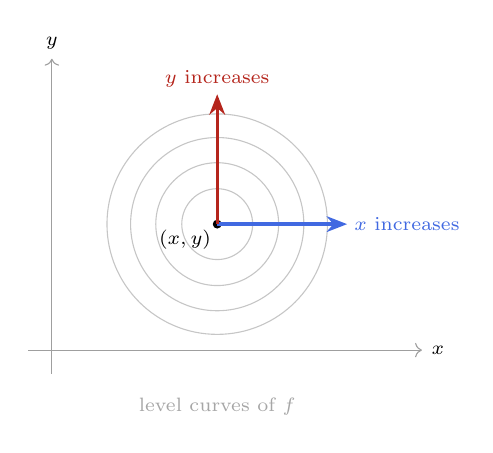
\begin{tikzpicture}[scale=1.0]
  \draw[axisline] (-0.3,0) -- (4.7,0) node[right,font=\scriptsize,black]{$x$};
  \draw[axisline] (0,-0.3) -- (0,3.7) node[above,font=\scriptsize,black]{$y$};
  \foreach \r in {0.45,0.78,1.10,1.40}
    { \draw[gray!45] (2.1,1.6) circle (\r); }
  \fill[black] (2.1,1.6) circle (1.6pt);
  \node[below left,font=\scriptsize,inner sep=2pt] at (2.1,1.6) {$(x,y)$};
  \draw[vecarr,RoyalBlue] (2.1,1.6) -- (3.75,1.6)
        node[right,font=\scriptsize,inner sep=2pt]{$x$ increases};
  \draw[vecarr,BrickRed]  (2.1,1.6) -- (2.1,3.25)
        node[above,font=\scriptsize,inner sep=2pt]{$y$ increases};
  \node[font=\scriptsize,gray!70] at (2.1,-0.72) {level curves of $f$};
\end{tikzpicture}
\end{center}

\noindent Each arrow is one partial derivative: step off the point along one
coordinate axis, and measure the rate at which $f$ responds.

%------------------------------------------------------------------------------
\subsection{What they look like on the surface}
%------------------------------------------------------------------------------
The picture above is drawn in the plane, where the function lives as a set of
level curves. The more telling picture is drawn on the graph.

Fix the point $(a,b)$ and hold $y$ at the value $b$. The set of points with
$y=b$ is a line in the plane; sitting above it on the surface $z=f(x,y)$ is a
single curve --- the \textbf{slice} of the surface cut by the vertical plane
$y=b$. Along that curve only $x$ varies, so it is the graph of the one-variable
function
\[
  g(x) \;=\; f(x,b) .
\]
And $\partial f/\partial x(a,b)$ is exactly $g'(a)$: the ordinary slope of the
tangent line to that slice, at that point.

\begin{center}
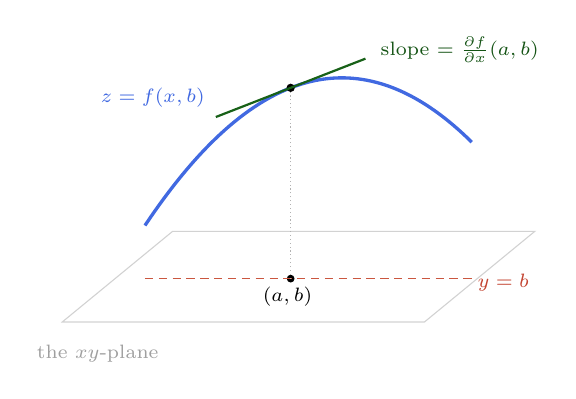
\begin{tikzpicture}[scale=1.0]
  % --- the surface, suggested by a patch and two slice curves -------------
  % base plane, drawn in a shallow oblique projection
  \draw[gray!35] (0,0) -- (4.6,0) -- (6.0,1.15) -- (1.4,1.15) -- cycle;
  \node[font=\scriptsize,gray!75] at (0.45,-0.40) {the $xy$-plane};
  % the point (a,b) in the base plane
  \coordinate (B) at (2.9,0.55);
  \fill[black] (B) circle (1.4pt);
  \node[below,font=\scriptsize,inner sep=1.5pt] at (2.86,0.50) {$(a,b)$};
  % the line y = b in the base plane
  \draw[BrickRed!70,densely dashed] (1.05,0.55) -- (5.2,0.55);
  \node[right,font=\scriptsize,BrickRed!80] at (5.15,0.50) {$y=b$};
  % the slice curve, lifted above that line
  \draw[curveln,domain=1.05:5.2,smooth,samples=70]
        plot (\x,{0.55 + 2.55 - 0.30*(\x-3.55)*(\x-3.55)});
  \node[font=\scriptsize,RoyalBlue] at (1.15,2.85) {$z=f(x,b)$};
  % the point on the curve above (a,b), and its tangent
  \coordinate (P) at (2.9,{0.55+2.55-0.30*(2.9-3.55)*(2.9-3.55)});
  \fill[black] (P) circle (1.5pt);
  \draw[gray!60,densely dotted] (B) -- (P);
  % slope of the slice at x=2.9 is -0.60*(2.9-3.55) = 0.39
  \draw[ForestGreen!70!black,thick]
        (1.95,{0.55+2.55-0.30*0.4225-0.39*0.95}) --
        (3.85,{0.55+2.55-0.30*0.4225+0.39*0.95});
  \node[right,font=\scriptsize,ForestGreen!60!black] at (3.92,3.46)
        {slope $=\pd{f}{x}(a,b)$};
\end{tikzpicture}
\end{center}

\noindent Holding $x$ at $a$ instead cuts the surface with the plane $x=a$,
producing a different curve, and $\partial f/\partial y(a,b)$ is the slope of
\emph{its} tangent at the same point. Two planes through one point of the
surface, two curves, two slopes.

\begin{rmk}
This is why a single number cannot be ``the slope'' of a surface. The surface
has a different slope in every direction you slice it, and the two partial
derivatives report only the two slices lined up with the axes. \S8 asks what
happens along all the other slices.
\end{rmk}

%------------------------------------------------------------------------------
\subsection{Computing them}
%------------------------------------------------------------------------------
In practice the limit is never evaluated. Since the other variable is held
fixed, it behaves as a constant, and the expression becomes a function of the
one live variable --- so the rules of \S2 apply unchanged.

\begin{center}
\fcolorbox{RoyalBlue!45}{RoyalBlue!7}{%
\begin{minipage}{0.9\textwidth}
\centering
To compute $\partial f/\partial x$: treat $y$ as a constant, and differentiate
as in one-variable calculus. To compute $\partial f/\partial y$: treat $x$ as a
constant and do the same.
\end{minipage}}
\end{center}

\begin{ex}
Let $f(x,y)=x^{2}y+3y^{2}$.

For $\partial f/\partial x$, treat $y$ as a constant. Then $x^{2}y$ is a
constant times $x^{2}$, and $3y^{2}$ is a constant, whose derivative is zero:
\[
  \pd{f}{x}=2xy .
\]
For $\partial f/\partial y$, treat $x$ as a constant. Now $x^{2}y$ is a constant
times $y$, and $3y^{2}$ is live:
\[
  \pd{f}{y}=x^{2}+6y .
\]
\end{ex}

\begin{ex}
Let $f(x,y)=e^{-(x^{2}+y^{2})}$, example (e) of \S5.2. By the chain rule,
holding $y$ fixed,
\[
  \pd{f}{x}=e^{-(x^{2}+y^{2})}\cdot(-2x)=-2x\,e^{-(x^{2}+y^{2})},
  \qquad
  \pd{f}{y}=-2y\,e^{-(x^{2}+y^{2})} .
\]
The two are the same computation with the roles of $x$ and $y$ exchanged, which
they must be: the formula for $f$ is unchanged by that exchange.
\end{ex}

\begin{ex}
Let $f(x,y)=x^{3}\ln y + \dfrac{y}{x}$, for $x\neq0$ and $y>0$. Holding $y$
fixed, $\ln y$ is a constant multiplier and $y/x=y\cdot x^{-1}$:
\[
  \pd{f}{x} = 3x^{2}\ln y - \frac{y}{x^{2}} .
\]
Holding $x$ fixed, $x^{3}$ is a constant multiplier, $\tfrac{d}{dy}\ln y=1/y$ by
\S4.1, and $y/x$ is a constant times $y$:
\[
  \pd{f}{y} = \frac{x^{3}}{y} + \frac{1}{x} .
\]
\end{ex}

\begin{ex}
Let $f(x,y)=\sin(xy)$. Holding $y$ fixed, the inside function is $xy$, whose
derivative with respect to $x$ is $y$; the chain rule gives
\[
  \pd{f}{x}=y\cos(xy),
  \qquad\text{and symmetrically}\qquad
  \pd{f}{y}=x\cos(xy) .
\]
Note that the held variable does not disappear --- it survives as a factor,
because it was a coefficient of the live variable inside the sine.
\end{ex}

\begin{ex}
Let $f(\vc{x})=\ip{\vc{a}}{\vc{x}}=a_1x+a_2y$, example (d) of \S5.2, with
$\vc{a}=[\,a_1,\,a_2\,]$ fixed. Only the first term involves $x$, and in it $x$
appears to the first power with coefficient $a_1$; the second term is a
constant. So
\[
  \pd{f}{x}=a_1,
  \qquad
  \pd{f}{y}=a_2 .
\]
The partial derivatives of a dot product against $\vc{a}$ are the components of
$\vc{a}$ itself.
\end{ex}

%------------------------------------------------------------------------------
\subsection{What kind of object is a partial derivative?}
%------------------------------------------------------------------------------
This is worth stating carefully, because it is what the next section is built
on.

At each point $(x,y)\in\R^{2}$, the limit \eqref{eq:partialx} produces a single
number. So $\partial f/\partial x$ assigns one real number to each point of the
plane --- which is to say it is itself a function
\[
  \pd{f}{x}:\R^{2}\longrightarrow\R ,
\]
of exactly the same type as $f$. Differentiating with respect to one variable
does not reduce the number of variables; the results above are visibly still
functions of both $x$ and $y$.

And there are two of them.

%==============================================================================
\section{The gradient}
%==============================================================================

%------------------------------------------------------------------------------
\subsection{Collecting the partials}
%------------------------------------------------------------------------------
So a single function $f:\R^{2}\to\R$ does not have \emph{a} derivative. It has
two --- one per coordinate direction --- and each is a function $\R^{2}\to\R$ in
its own right. Naming and carrying them separately would obscure the fact that
they belong together: they are two answers to the same question, asked in two
directions.

\lookback The vector unit's opening move was exactly this. Faced with several
related numbers, do not track them separately --- package them into a single
object of $\R^{2}$ and work with that. Position, velocity and force were treated
that way.

Apply that move here.

\begin{defn}[Gradient]
Let $f:\R^{2}\to\R$ have both partial derivatives at $\vc{x}=(x,y)$. The
\textbf{gradient} of $f$ at $\vc{x}$ is the vector in $\R^{2}$ whose components
are the two partial derivatives:
\[
  \grad f(\vc{x})
  \;=\;
  \left[\;\pd{f}{x}(x,y),\;\;\pd{f}{y}(x,y)\;\right] .
\]
\end{defn}

\noindent The symbol $\grad$ is read ``del'' or ``nabla''. Note the signature
that results:
\[
  f:\R^{2}\to\R,
  \qquad\text{but}\qquad
  \grad f:\R^{2}\to\R^{2} .
\]
The gradient takes a point and returns a \emph{vector}. This is a genuine
departure from the one-variable case, where $f'$ had the same signature as $f$.

%------------------------------------------------------------------------------
\subsection{Examples}
%------------------------------------------------------------------------------
\begin{ex}
For $f(x,y)=x^{2}y+3y^{2}$, the partials were computed in \S6.3, so
\[
  \grad f(x,y)=\bigl[\,2xy,\;\;x^{2}+6y\,\bigr] .
\]
At the point $(1,2)$ this evaluates to $\grad f(1,2)=[\,4,\,13\,]$ --- a vector
in $\R^{2}$ attached to that particular point. At a different point it is a
different vector: $\grad f(0,1)=[\,0,\,6\,]$, and $\grad f(-1,0)=[\,0,\,1\,]$.
\end{ex}

\begin{ex}
For $f(x,y)=x^{2}+y^{2}$,
\[
  \grad f(x,y)=[\,2x,\,2y\,]=2\,[\,x,\,y\,] .
\]
At every point the gradient is twice the position vector, so it points directly
away from the origin --- which is where $f$ is smallest. That is the first hint
of \S8.
\end{ex}

\begin{ex}
For $f(x,y)=\sin(xy)$, the partials were $y\cos(xy)$ and $x\cos(xy)$, so
\[
  \grad f(x,y) = \cos(xy)\,[\,y,\,x\,] .
\]
Here the gradient happens to factor: a scalar depending on the point, times a
vector. At $(\pi,\tfrac12)$, $\cos(\pi/2)=0$, so $\grad f=[\,0,\,0\,]$ --- the
gradient is the zero vector there, and $f$ is momentarily flat in \emph{both}
coordinate directions.
\end{ex}

\begin{ex}
For $f(\vc{x})=\ip{\vc{a}}{\vc{x}}$, the last example of \S6.3 gave
$\partial f/\partial x=a_1$ and $\partial f/\partial y=a_2$. Assembling them,
\[
  \grad f(\vc{x}) = [\,a_1,\,a_2\,] = \vc{a} .
\]
The gradient is $\vc{a}$ itself, the same at every point --- the two-variable
counterpart of the fact that a line of slope $m$ has derivative $m$ everywhere.
\end{ex}

\begin{rmk}[Why this is the right package]
Collecting the two partials into a vector could look like mere bookkeeping. It
is more than that, for a reason visible in the last example: the gradient of
$\ip{\vc{a}}{\vc{x}}$ came out as $\vc{a}$, not as two unrelated numbers that
happen to be stored together. The package has an identity of its own. And
because $\grad f(\vc{x})$ is a vector in $\R^{2}$, everything the vector unit
built applies to it: it has a length, it has a direction, it can be dotted with
other vectors, it can be normalised, and it can be tested for orthogonality. The
next section spends every one of those.
\end{rmk}

%==============================================================================
\section{The directional derivative, and steepest ascent}
%==============================================================================
\S5.3 left a question open: the rate of change of $f$ at a point is not
well-posed until a direction is named, and \S6 named only two of them. This
section names all of them at once, and then asks which one is best.

%------------------------------------------------------------------------------
\subsection{The idea}
%------------------------------------------------------------------------------
Stand at a point $\vc{x}$ of the plane and pick a direction to walk in. A
direction is a vector $\vc{u}$, and the natural question is: \emph{as I set off
that way, how fast does $f$ change?}

That number depends on two things, and on nothing else: the point you are
standing at, and the direction you chose. Give it a name.

\begin{center}
\fcolorbox{RoyalBlue!45}{RoyalBlue!7}{%
\begin{minipage}{0.9\textwidth}
\centering
The \textbf{directional derivative} $D_{\vc{u}}f(\vc{x})$ is the rate of change
of $f$ at the point $\vc{x}$, in the direction of the vector $\vc{u}$.
\end{minipage}}
\end{center}

\noindent Said as a limit, it is \eqref{eq:deriv} once more, with the step
$h\vc{u}$ --- a step of size $h$ taken \emph{in the direction $\vc{u}$}:
\begin{equation}\label{eq:dirderiv}
  D_{\vc{u}}f(\vc{x})
  \;=\;
  \lim_{h\to0}\frac{f(\vc{x}+h\vc{u})-f(\vc{x})}{h} .
\end{equation}
Every definition so far is a special case. Taking $\vc{u}=[\,1,\,0\,]$ makes
$\vc{x}+h\vc{u}=(x+h,\,y)$, and \eqref{eq:dirderiv} becomes
\eqref{eq:partialx}. Taking $\vc{u}=[\,0,\,1\,]$ gives \eqref{eq:partialy}.
The two partial derivatives are the directional derivative in the two
directions we happened to name first.

\begin{warn}[Take $\vc{u}$ to have length one]
$D_{\vc{u}}f$ is meant to measure a rate \emph{per unit of distance travelled},
so the direction vector must be a unit vector --- otherwise doubling the length
of $\vc{u}$ doubles the answer without any change of direction, and the number
measures the arrow rather than the hillside. Whenever a direction is given as a
vector that is not already of length one, normalise it first:
$\vc{u}=\vc{v}/\norm{\vc{v}}$, as in \S12.1 of the vector unit. Both
$[\,1,\,0\,]$ and $[\,0,\,1\,]$ above are unit vectors, as they had to be.
\end{warn}

%------------------------------------------------------------------------------
\subsection{Computing it from the gradient}
%------------------------------------------------------------------------------
The limit \eqref{eq:dirderiv} is no more pleasant to evaluate than any other, and
it does not have to be. The gradient already holds the answer.

Walking in the direction $\vc{u}=[\,u_1,\,u_2\,]$ means changing $x$ at rate
$u_1$ and changing $y$ at rate $u_2$, at the same time. Each partial derivative
is the exchange rate for its own coordinate --- $\partial f/\partial x$ says how
much $f$ moves per unit of $x$ --- so the contribution from the $x$-motion is
$\pd{f}{x}u_1$, the contribution from the $y$-motion is $\pd{f}{y}u_2$, and the
total rate is their sum:
\[
  D_{\vc{u}}f(\vc{x})
  \;=\; \pd{f}{x}(\vc{x})\,u_1 + \pd{f}{y}(\vc{x})\,u_2 .
\]
That sum of products of matching components is a dot product, and the vector it
is taken against is the gradient.

\begin{center}
\fcolorbox{RoyalBlue!45}{RoyalBlue!7}{%
\begin{minipage}{0.9\textwidth}
\centering
For a unit vector $\vc{u}$,
\[
  D_{\vc{u}}f(\vc{x}) \;=\; \ip{\grad f(\vc{x})}{\vc{u}} .
\]
\end{minipage}}
\end{center}

\noindent This is the first place the gradient pays for itself. The two
partials answered two questions; packaged as a vector and dotted against
$\vc{u}$, they answer all of them.

\begin{rmk}
The argument just given is a motivation, not a proof --- it assumes that the
separate coordinate effects simply add, which is the content of the linear
approximation of \S9.2. Taking that formula as the definition of how $f$ behaves
near $\vc{x}$, the identity above is immediate; \S9.2 closes the loop.
\end{rmk}

\begin{ex}
Let $f(x,y)=x^{2}y+3y^{2}$ and take the point $(1,2)$, where $\S7.2$ gave
$\grad f(1,2)=[\,4,\,13\,]$. Find the rate of change of $f$ there in the
direction of $\vc{v}=[\,3,\,4\,]$.

First normalise: $\norm{\vc{v}}=\sqrt{9+16}=5$, so
$\vc{u}=\tfrac15[\,3,\,4\,]=[\,\tfrac35,\,\tfrac45\,]$. Then
\[
  D_{\vc{u}}f(1,2)
  = \bigl\langle[\,4,\,13\,],\;[\,\tfrac35,\,\tfrac45\,]\bigr\rangle
  = \frac{12}{5}+\frac{52}{5}
  = \frac{64}{5} = 12.8 .
\]
Positive, so $f$ increases as you set off that way.
\end{ex}

\begin{ex}
Same $f$ and same point, but in the direction $\vc{v}=[\,-13,\,4\,]$. Here
$\norm{\vc{v}}=\sqrt{169+16}=\sqrt{185}$, and
\[
  D_{\vc{u}}f(1,2)
  = \frac{1}{\sqrt{185}}\bigl\langle[\,4,\,13\,],\,[\,-13,\,4\,]\bigr\rangle
  = \frac{-52+52}{\sqrt{185}} = 0 .
\]
The rate is zero: walking that way, $f$ does not change at all to first order.
By the orthogonality test of the vector unit's \S11.7, that happened precisely
because $[\,-13,\,4\,]$ is orthogonal to the gradient --- and the directions
orthogonal to $\grad f$ are the ones along which $f$ holds still. Those are the
level curves.
\end{ex}

%------------------------------------------------------------------------------
\subsection{In which direction is the rate of change greatest?}
%------------------------------------------------------------------------------
Now the question worth asking. Standing at $\vc{x}$, every unit vector $\vc{u}$
gives some rate $D_{\vc{u}}f(\vc{x})$. \emph{Which $\vc{u}$ makes it as large as
possible?}

Write the formula of \S8.2 and then rewrite the dot product the way the vector
unit's \S11.3 does, in terms of the angle $\theta$ between $\grad f(\vc{x})$ and
$\vc{u}$:
\begin{equation}\label{eq:steepest}
  D_{\vc{u}}f(\vc{x})
  \;=\; \ip{\grad f(\vc{x})}{\vc{u}}
  \;=\; \norm{\grad f(\vc{x})}\,\norm{\vc{u}}\cos\theta
  \;=\; \norm{\grad f(\vc{x})}\cos\theta ,
\end{equation}
the last step because $\norm{\vc{u}}=1$.

Read what \eqref{eq:steepest} says. As $\vc{u}$ swings around the point, the
factor $\norm{\grad f(\vc{x})}$ does not move --- it is fixed by the point, not
by the direction. The \emph{only} thing that varies is $\cos\theta$, and
$\cos\theta$ is largest, equal to $1$, exactly when $\theta=0$. So the rate is
greatest when the angle between $\vc{u}$ and the gradient is zero: when $\vc{u}$
points the same way as $\grad f(\vc{x})$.

There is exactly one unit vector that does that. Assuming
$\grad f(\vc{x})\neq\vc{0}$, take
\[
  \vc{u} \;=\; \frac{\grad f(\vc{x})}{\norm{\grad f(\vc{x})}} ,
\]
the normalisation of the gradient (vector unit \S12.1). Substituting it into the
formula of \S8.2 confirms the value:
\[
  D_{\vc{u}}f(\vc{x})
  = \left\langle \grad f(\vc{x}),\;
      \frac{\grad f(\vc{x})}{\norm{\grad f(\vc{x})}}\right\rangle
  = \frac{\ip{\grad f(\vc{x})}{\grad f(\vc{x})}}{\norm{\grad f(\vc{x})}}
  = \frac{\norm{\grad f(\vc{x})}^{2}}{\norm{\grad f(\vc{x})}}
  = \norm{\grad f(\vc{x})} ,
\]
using $\ip{\vc{w}}{\vc{w}}=\norm{\vc{w}}^{2}$ from the vector unit's \S11.6.

So the rate of change at $\vc{x}$ is maximal along the direction of
$\grad f(\vc{x})$, and the maximal rate is $\norm{\grad f(\vc{x})}$. Since that
value is positive, $f$ genuinely increases in that direction: the gradient is an
\emph{ascent} direction, and no direction ascends faster.

\begin{center}
\fcolorbox{RoyalBlue!45}{RoyalBlue!7}{%
\begin{minipage}{0.9\textwidth}
\centering
At a point $\vc{x}$ where both partial derivatives exist and
$\grad f(\vc{x})\neq\vc{0}$, the gradient $\grad f(\vc{x})$ points in the
direction of \textbf{steepest ascent} of $f$, and its length
$\norm{\grad f(\vc{x})}$ is the rate of climb in that direction.
\end{minipage}}
\end{center}

\begin{rmk}[The two extremes, and the flat directions]
The same reading of \eqref{eq:steepest} settles the other cases at no extra
cost. $\cos\theta$ is smallest, equal to $-1$, when $\theta=\pi$ --- so the rate
is \emph{most negative} when $\vc{u}$ points opposite to the gradient, and
$-\grad f(\vc{x})$ is the direction of \textbf{steepest descent}. And
$\cos\theta=0$ when $\theta=\pi/2$, so the rate is zero exactly along the
directions orthogonal to the gradient, which is what the second example of
\S8.2 found by arithmetic. Those are the directions in which $f$ holds still:
the gradient crosses the level curves of $f$ at right angles.
\end{rmk}

\begin{center}
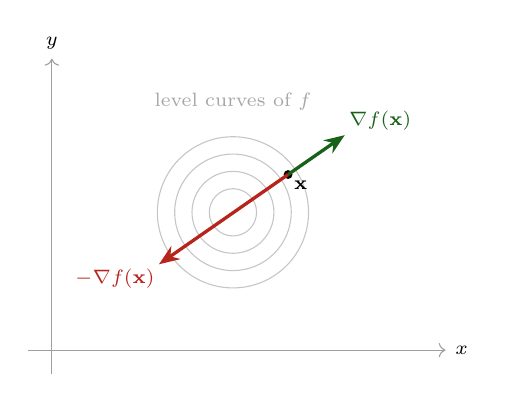
\begin{tikzpicture}[scale=1.0]
  \draw[axisline] (-0.3,0) -- (5.0,0) node[right,font=\scriptsize,black]{$x$};
  \draw[axisline] (0,-0.3) -- (0,3.7) node[above,font=\scriptsize,black]{$y$};
  \foreach \r in {0.30,0.52,0.74,0.96}
    { \draw[gray!45] (2.3,1.75) circle (\r); }
  \node[font=\scriptsize,gray!70] at (2.3,3.15) {level curves of $f$};
  \coordinate (P) at (3.0,2.23);
  \fill[black] (P) circle (1.6pt);
  \node[below right,font=\scriptsize,inner sep=2pt] at (P) {$\vc{x}$};
  \draw[vecarr,ForestGreen!70!black] (P) -- (3.72,2.73)
        node[above right,font=\scriptsize,inner sep=1pt]{$\grad f(\vc{x})$};
  \draw[vecarr,BrickRed] (P) -- (1.36,1.09)
        node[below left,font=\scriptsize,inner sep=1pt]{$-\grad f(\vc{x})$};
\end{tikzpicture}
\end{center}

\noindent The two arrows show \emph{directions}; their drawn lengths are not to
scale. The gradient heads toward the level curves where $f$ is larger. Reversing
it gives the direction of steepest descent --- here, straight toward the low
point at the centre.

\begin{rmk}[The same thing happens in one variable]
With one variable there are only two directions to move, and the gradient is the
single number $f'(x)$. If $f'(x)>0$ then $f$ increases as $x$ increases, so
``uphill'' is the positive direction; if $f'(x)<0$, uphill is the negative
direction. In both cases uphill is the direction the derivative points, and
$\lvert f'(x)\rvert$ says how steep the slope is. The gradient is that statement
with more than two directions available --- which is why it must be a vector
rather than a sign.
\end{rmk}

%------------------------------------------------------------------------------
\subsection{Gradient descent}
%------------------------------------------------------------------------------
The descent half of the last remark is the more useful one in practice, because
most problems worth solving are phrased as \emph{make this quantity small}.

Suppose $f(x,y)$ measures how badly something is performing --- the error of a
prediction, the cost of a design --- and you want the $(x,y)$ that makes it as
small as possible. You cannot see the whole surface. But at whatever point you
are standing, you can compute $\grad f$, and $-\grad f$ tells you which way is
downhill, faster than any other way. So: step that way, and repeat.
\[
  \vc{x}_{k+1} \;=\; \vc{x}_{k} \;-\; \alpha\,\grad f(\vc{x}_k),
  \qquad \alpha>0 .
\]
The number $\alpha$ is the \textbf{step size}, controlling how far to move
before recomputing. This is \textbf{gradient descent}, and it is the workhorse
of modern optimisation and machine learning --- the method by which very nearly
every neural network in existence is trained. It exists because of the boxed
statement in \S8.3 and nothing more.

\lookahead Two questions are already visible. The iteration stops making
progress where $\grad f=\vc{0}$, so those points deserve a name and a study ---
they are the candidates for maxima and minima. And knowing only the slope,
gradient descent has no idea whether the ground ahead curves up or down, so it
cannot tell how big a step is safe; answering that needs a \emph{second}
derivative, which in more than one variable is neither a number nor a vector.
Part 2 of this unit takes both up.

%==============================================================================
\section{Linear approximation}
%==============================================================================
One of the oldest uses of a derivative is to replace a complicated function, near
a single point, by a simple one. The gradient does this in the plane exactly as
$f'$ does on the line --- and comparing the two formulas shows what kind of
object the gradient really is.

%------------------------------------------------------------------------------
\subsection{One variable}
%------------------------------------------------------------------------------
Return to the picture in \S1.1. The tangent line at $x=a$ touches the graph at
that point and has slope $f'(a)$, so its equation is
\begin{equation}\label{eq:lin1}
  L(x) \;=\; f(a) + f'(a)\,(x-a) .
\end{equation}
Near $a$ the curve and its tangent line are hard to tell apart, so $L$ can stand
in for $f$:
\[
  f(x) \;\approx\; f(a) + f'(a)\,(x-a)
  \qquad\text{for } x \text{ near } a .
\]
This is the \textbf{linear approximation} (or \emph{linearisation}) of $f$ at
$a$. Read \eqref{eq:lin1} in three pieces: start from the known value $f(a)$,
measure how far you have moved with $x-a$, and convert that displacement into a
change in $f$ by multiplying by the rate $f'(a)$.

\begin{ex}
Estimate $\sqrt{4.1}$ without a calculator. Take $f(x)=\sqrt{x}$ and $a=4$,
where the value is known exactly. Then $f(4)=2$ and
$f'(x)=\tfrac{1}{2\sqrt{x}}$, so $f'(4)=\tfrac14$. Hence
\[
  \sqrt{4.1}\;\approx\; 2 + \tfrac14(4.1-4) = 2 + \tfrac{0.1}{4} = 2.025 .
\]
The true value is $2.02484\ldots$, so the estimate is off by about $1.5\times
10^{-4}$ --- from arithmetic done in one line.
\end{ex}

%------------------------------------------------------------------------------
\subsection{Two variables}
%------------------------------------------------------------------------------
Now let $f:\R^{2}\to\R$ and let $\vc{a}=(a_1,a_2)$ be the point we are near.
Every piece of \eqref{eq:lin1} survives, but two of them change type.

The starting value $f(\vc{a})$ is still a scalar. The displacement is now
$\vc{x}-\vc{a}$, a \emph{vector} --- it must record how far we moved in both
coordinates, not just one. And the rate is now $\grad f(\vc{a})$, also a vector.
To turn a vector of rates and a vector of displacements into a single number,
there is exactly one natural operation available, and the vector unit built it:
the dot product.

\begin{defn}[Linear approximation in two variables]
Let $f:\R^{2}\to\R$ have a gradient at $\vc{a}$. The \textbf{linear
approximation} of $f$ at $\vc{a}$ is
\begin{equation}\label{eq:lin2}
  L(\vc{x}) \;=\; f(\vc{a}) + \ip{\grad f(\vc{a})}{\;\vc{x}-\vc{a}} ,
\end{equation}
and $f(\vc{x})\approx L(\vc{x})$ for $\vc{x}$ near $\vc{a}$.
\end{defn}

\noindent Set the two formulas side by side:
\[
  \underbrace{f(a) + f'(a)\,(x-a)}_{\text{one variable}}
  \qquad\longleftrightarrow\qquad
  \underbrace{f(\vc{a}) + \ip{\grad f(\vc{a})}{\vc{x}-\vc{a}}}_{\text{two variables}} .
\]
They are the same formula. The only change is that a product of two numbers has
become a dot product of two vectors.

Written out in coordinates, \eqref{eq:lin2} reads
\[
  L(x,y) = f(a_1,a_2)
    + \pd{f}{x}(\vc{a})\,(x-a_1)
    + \pd{f}{y}(\vc{a})\,(y-a_2) ,
\]
one term per direction: each partial derivative converts the displacement in its
own coordinate into a contribution to the change in $f$, and the two
contributions are added.

\begin{ex}
Let $f(x,y)=x^{2}+y^{2}$ and approximate near $\vc{a}=(1,2)$. There
$f(\vc{a})=1+4=5$, and from \S7.2, $\grad f(x,y)=[\,2x,\,2y\,]$, so
$\grad f(\vc{a})=[\,2,\,4\,]$. Then
\[
  L(x,y) = 5 + \bigl\langle[\,2,4\,],\,[\,x-1,\;y-2\,]\bigr\rangle
         = 5 + 2(x-1) + 4(y-2) .
\]
At $(1.1,\,1.9)$ this predicts
\[
  L(1.1,1.9) = 5 + 2(0.1) + 4(-0.1) = 5 + 0.2 - 0.4 = 4.8 ,
\]
against the true value $1.21+3.61=4.82$. Note the two terms pulling opposite
ways: moving right raises $f$, moving down lowers it, and the approximation adds
both effects.
\end{ex}

\begin{rmk}[What the graph of $L$ is]
For one variable the linear approximation is a tangent \emph{line}. For two it
is a tangent \emph{plane}, resting on the surface at a single point. In both
cases it is the flat object that best matches $f$ at $\vc{a}$ --- and it is the
same plane whose slices, in the two coordinate directions, are the tangent lines
drawn in \S6.2.
\end{rmk}

\begin{rmk}[Why the gradient deserves to be called the derivative]
\eqref{eq:lin2} is the strongest answer to the question of what replaces $f'$ in
two variables. In one variable, $f'(a)$ is the number that makes the best linear
approximation work. In two, $\grad f(\vc{a})$ is the vector that plays that role
--- the same job, the same position in the formula, a different type of object.
Collecting the partials into a vector was not bookkeeping after all: it produced
the thing that behaves like a derivative.
\end{rmk}

\begin{rmk}[And it closes the loop of \S8.2]
Put $\vc{x}=\vc{a}+h\vc{u}$ into \eqref{eq:lin2}, so that the displacement is
$h\vc{u}$. The dot product is linear in that slot, so
\[
  L(\vc{a}+h\vc{u}) = f(\vc{a}) + h\,\ip{\grad f(\vc{a})}{\vc{u}} ,
\]
and the change in the approximation, divided by the distance $h$ travelled, is
$\ip{\grad f(\vc{a})}{\vc{u}}$ --- exactly the directional derivative claimed in
\S8.2. The formula asserted there is the linear approximation read along a
single direction.
\end{rmk}

\lookahead Two roads lead out of here. Asking where $L$ is flat --- where
$\grad f(\vc{a})=\vc{0}$ --- locates the candidates for maxima and minima, the
points at which gradient descent stalls. And approximating with something better
than a flat object requires a \emph{second} derivative, which for a function of
two variables turns out to be neither a number nor a vector but a
\emph{matrix}. Both belong to Part 2, which also lifts everything in \S5--\S9
from the plane to $\R^{n}$.

\end{document}
